\chapter{Discussion}

This chapter provides an in-depth analysis of the experimental results, focusing on two performance metrics demonstrated by the robot under the SMC control strategy:  path efficiency and computation time. Each metric is evaluated in detail to analyze the strengths and limitations of the Sliding Mode Control (SMC) algorithm in navigation and obstacle avoidance tasks.


\section{Path Efficiency}

Path efficiency is an important metric for evaluating the performance of the Sliding Mode Control (SMC) algorithm. Ideally, the robot should follow the shortest path from the starting point to the target. However, due to the presence of obstacles, different control strategies are employed to guide the robot in avoiding obstacles and reaching the target. The path lengths resulting from different strategies vary. This section provides a comparative analysis of the path length achieved by the SMC strategy against the shortest possible path.

As shown in Figure~\ref{fig:shortest_path}, the shortest path is a straight line connecting the start and target positions. Its length can be calculated using the following formula:
\begin{equation}
L_{\text{shortest}} = \sqrt{(x_{\text{goal}} - x_{\text{start}})^2 + (y_{\text{goal}} - y_{\text{start}})^2}
\end{equation}
where $(x_{\text{start}}, y_{\text{start}})$ and $(x_{\text{goal}}, y_{\text{goal}})$ represent the coordinates of the start and target positions, respectively. In this experiment, the start position is $(0, 0)$, and the target position is $(5, 4)$. Substituting these values yields:
\begin{equation}
L_{\text{shortest}} = \sqrt{(5 - 0)^2 + (4 - 0)^2} = \sqrt{25 + 16} = 6.4 \, \text{units}
\end{equation}

\begin{figure}[ht]
    \centering
    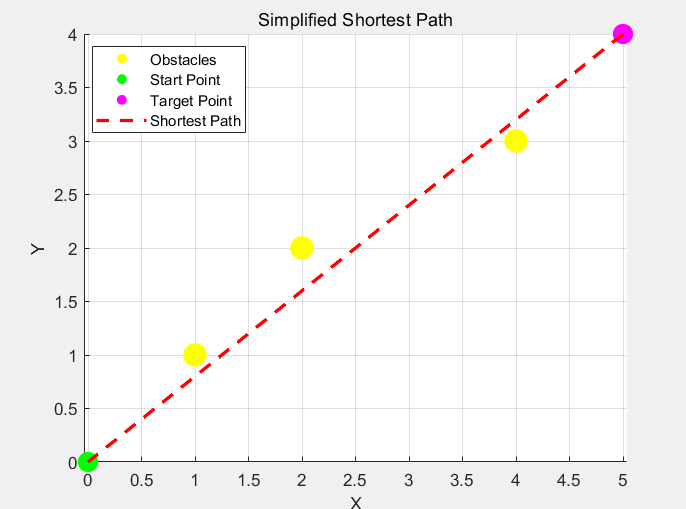
\includegraphics[width=0.6\textwidth]{image/12.PNG}
    \caption{Shortest path connecting the start and target positions}
    \label{fig:shortest_path}
\end{figure}

In contrast, the actual path length is calculated by summing the distances between successive points in the robot's trajectory. As illustrated in Figure~\ref{FIG:7}, the robot's trajectory, generated by the SMC algorithm, avoids obstacles and ultimately reaches the target. The trajectory is recorded as a sequence of discrete points $(x_1, y_1), (x_2, y_2), \dots, (x_n, y_n)$, and the actual path length is computed as:
\begin{equation}
L_{\text{actual}} = \sum_{i=1}^{n-1} \sqrt{(x_{i+1} - x_i)^2 + (y_{i+1} - y_i)^2}
\end{equation}
Using this formula and the recorded trajectory, the actual path length was determined to be:
\begin{equation}
L_{\text{actual}} = 7.6 \, \text{units}
\end{equation}

Path efficiency is defined as the ratio of the shortest path length to the actual path length:
\begin{equation}
\text{Path Efficiency} = \frac{L_{\text{shortest}}}{L_{\text{actual}}}
\end{equation}
Substituting the values obtained:
\begin{equation}
\text{Path Efficiency} = \frac{6.4}{7.6} \approx 0.842
\end{equation}

The results demonstrate that the SMC algorithm effectively maintains high path efficiency while avoiding obstacles. Although the actual path length is approximately \(18.75\%\) longer than the shortest path, this deviation is primarily due to the robot's detours to maintain a safe distance from obstacles. For most of the navigation process, the robot aligns its movement towards the target, achieving a reasonable balance between goal-directed behavior and collision avoidance.

\section{Computation Time}

Computation time is a critical metric for evaluating the real-time performance of navigation algorithms. This section presents the computation time required to complete the navigation tasks in both scenarios.

\subsubsection{Static Obstacle Navigation}

In the static obstacle scenario, the robot starts from the initial position (0, 0) and navigates to the target position (5, 4). The simulation parameters are set with a time step \(dt = 0.1\) and a maximum simulation time of 20 seconds. The total number of iterations can be calculated using the following formula:
\[
N = \frac{t_{\text{max}}}{dt} = \frac{20}{0.1} = 200 \, \text{steps}
\]

During navigation, the robot avoids obstacles while gradually approaching the target. According to the real-time display outputs, the robot reaches the target at step 77 with the following observations (Figure~\ref{fig:static_output}):

\begin{figure}[ht]
    \centering
    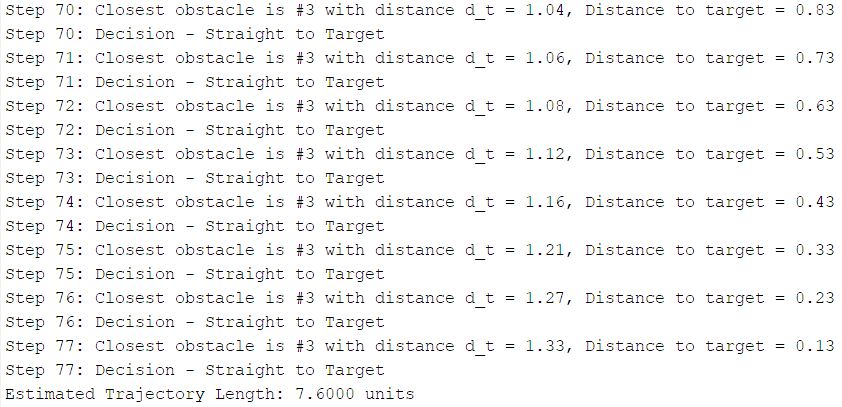
\includegraphics[width=0.8\textwidth]{13.png}
    \caption{Real-time outputs for the static obstacle scenario}
    \label{fig:static_output}
\end{figure}

In step 77, the robot is 1.33 units from the closest obstacle (Obstacle \#3) and 0.13 units from the target. At this point, the robot determines that it can move straight toward the target and completes the task. The total trajectory length is approximately \(7.600 \, \text{units}\). The task is completed in \(T_{\text{total}} = 7.7 \, \text{seconds}\). Figure~\ref{fig:static_output} illustrates the task completion process in the static obstacle scenario.


\subsubsection{Dynamic Obstacle Navigation}

In the dynamic obstacle scenario, the robot starts at \((0, 0)\) and navigates to a dynamic target located at \((3, 4)\). Dynamic obstacles move with constant velocity, increasing the complexity of the navigation task. The simulation parameters are the same as in the static scenario, with \(dt = 0.1\), \(t_{\text{max}} = 20\) seconds and 200 total steps.

The robot adjusts its path multiple times to avoid moving obstacles while gradually approaching the dynamic target. The real-time display outputs for steps 195 to 200 are as follows (Figure~\ref{fig:dynamic_output}):

\begin{figure}[ht]
    \centering
    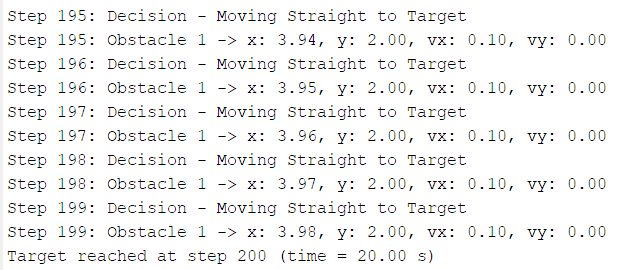
\includegraphics[width=0.8\textwidth]{14.png}
    \caption{Real-time outputs for the dynamic obstacle scenario}
    \label{fig:dynamic_output}
\end{figure}

In step 199, obstacle \#1 is located at \((3.98, 2.00)\) with a speed of \((v_x = 0.10, v_y = 0.00)\). The robot successfully reaches the target at step 200, completing the task in \(T_{\text{total}} = 20.0 \, \text{seconds}\). Figure~\ref{fig:dynamic_output} illustrates the task completion process in the dynamic obstacle scenario.


\subsubsection{Comparison and Discussion}

The comparison between static and dynamic obstacle scenarios reveals the impact of obstacle movement on navigation performance. In the dynamic scenario, the robot requires more adjustments to avoid moving obstacles, resulting in a longer task completion time. Table~\ref{tab:comparison} summarizes the task completion times and critical decision steps for both scenarios.


\begin{table}[H]
    \centering
    \caption{Comparison of static and dynamic obstacle navigation scenarios}
    \label{tab:comparison}
    \centering
    \begin{tabular}{|l|c|c|c|}
        \hline
        \textbf{Scenario} & \textbf{Total Step} & \textbf{Target Position} & \textbf{Decision Steps} \\ \hline
        Static Obstacle Navigation & 77 & (5, 4) & Step 77 \\ \hline
        Dynamic Obstacle Navigation & 200 & (3, 4) & Steps 200 \\ \hline
    \end{tabular}
\end{table}



\subsubsection{Summary}

The comparison shows that the SMC algorithm achieves a favorable computing time in the static obstacle environment. However, in the dynamic obstacle environment, the completion time significantly increases, reaching the maximum simulation duration. This increase in completion time is mainly due to frequent path adjustments and obstacle avoidance decisions in the dynamic obstacle environment.